\documentclass[10pt, a4paper]{article}

%Preambuła dokumentu
\usepackage{graphicx}
\usepackage{here}
\usepackage{rotating}
\usepackage{subfigure}
\usepackage{epic}
\usepackage{listings}
\usepackage{verbatim}
\usepackage{amssymb}
\usepackage{amsmath}
\usepackage[polish]{babel}
\usepackage[OT4]{fontenc}
\usepackage[utf8]{inputenc}

%\usepackage{here}

\textwidth      16cm
\textheight     25.5cm
\evensidemargin -3mm
\oddsidemargin  -3mm
\topmargin      -20mm



\author{Marcin Ciopcia \and Daniel Gut \and Piotr Semberecki \and Hanna Sienkiewicz \and Mateusz Stachowski
}
 
\title{Raport nr 1 z projektu Systemy Zdarzeniowe} 

\date{\today}

\begin{document}
\maketitle



\section{Problem Projektu}
\label{sec:wstep}
%
\subsection{Opis ogólny}
Pierwszym celem projektu jest symulacja zautomatyzowanej linii produkcyjnej z wieloma gniazdami wytwórczymi, obsługiwanej przez wózki AGV. Linia produkcyjna ma kształt pierścienia, z ustalonym dozwolonym kierunkiem ruchu wózków AGV, poruszających się jak na rysunku~\ref{fig:sch}.
 \begin{figure}[H]
  \begin{center}
    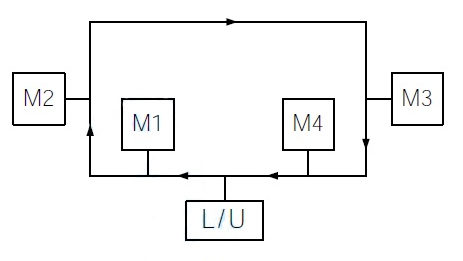
\includegraphics[width=0.3\textwidth]{./obrazki/Schemat.png}
    \caption{Struktura ścieżek}
    \label{fig:sch}
  \end{center}
 \end{figure}
Modelowany system posiada stacje załadowczo-rozładowczą (L/U), cztery stacje  maszynowe $(M_1,M_2,M_3,M_4)$, z których każda posiada bufor wejściowy i wyjściowy oraz robota wykonującego operację przeniesienia detalu z bufora wejściowego na stanowisko robocze maszyny oraz ze stanowiska roboczego do bufora wyjściowego. Opisywany system produkcyjny realizuje współbieżnie do sześciu typów produktów w podanej ilości. Operacje na danym produkcie zostają wykonane na rożnych maszynach w zadanej kolejności.
 
 
Następnie zostanie opracowany sterownik zdarzeniowy zarządzający logiką przepływu zadań w systemie składającą się z
\begin{itemize}
\item klasyfikatora zadań możliwych do realizacji,
\item systemu agentowego zarządzającego kolejnością wykonywania działań,
\item systemu przeciwdziałania zakleszczeniom zdarzeń w systemie.
\end{itemize}
Sterownik nadrzędny opisany zostanie za pomocą sieci Petriego, następnie zostanie oprogramowany w środowisku \textit{Matlab}.

\subsection{Zastosowanie systemów zdarzeniowych}
Podjęcie tego zagadnienie jest ważne ze względu na poszerzające się zastosowanie robotyzacji w wielu dziedzinach gospodarki. Za pomocą elastycznych komórek produkcyjnych (ESP) można modelować procesy produkcyjne, przepustowość sieci infrastruktury technicznej, systemy czasu rzeczywistego  \cite{scr} , sterowniki logiczne \cite{sl} czy sieć komunikacji miejskiej. Modele różnorodnych systemów pozwalają ocenić ich efektywność funkcjonowania \cite{mucha}, co może wpłynąć na zmniejszenie kosztów, niwelując błędy już przy projektowaniu danego systemu. Za pomocą systemów zdarzeniowych można modelować również poruszanie się robotów mobilnych, zapobiegając przy tym zakleszczeniom, kolizjom, optymalizując czas wykonania danego zadania czy przejazdu przez daną ścieżkę.

\subsection{Upowszechnienie wyników}

Wyniki projektu będą upowszechnione na serwisie www, który będzie zawierał
\begin{itemize}
\item archiwum z oprogramowaniem,
\item dokumentację algorytmów,
\item dokumentację oprogramowania dla użytkowników i deweloperów,
\item przykład działania systemu,
\item wyniki przeprowadzonych badań, w tym
\begin{itemize}
\item zbadanie poprawności działania systemu wykorzystując dostarczone dane wejściowe,
\item wpływ ilości robotów znajdujących się na maszynach
\item wpływ pojemności buforów wejściowch oraz wyjściowych maszyn na działanie systemu wpływ ilości robotów obsługujących operacje przeniesienia detalu z bufora wejściowego do miejsca operacyjnego maszyny jak i z miejsca operacyjnego maszyny do bufora wyjściowego na działanie systemu,
\item dobór algorytmu przeciwdziałającemu blokadom,
\item wpływ pojemności wózków AGV na działanie systemu.
\end{itemize}
\end{itemize}
\subsection{Sieć Petriego}

 \begin{figure}[H]
  \begin{center}
    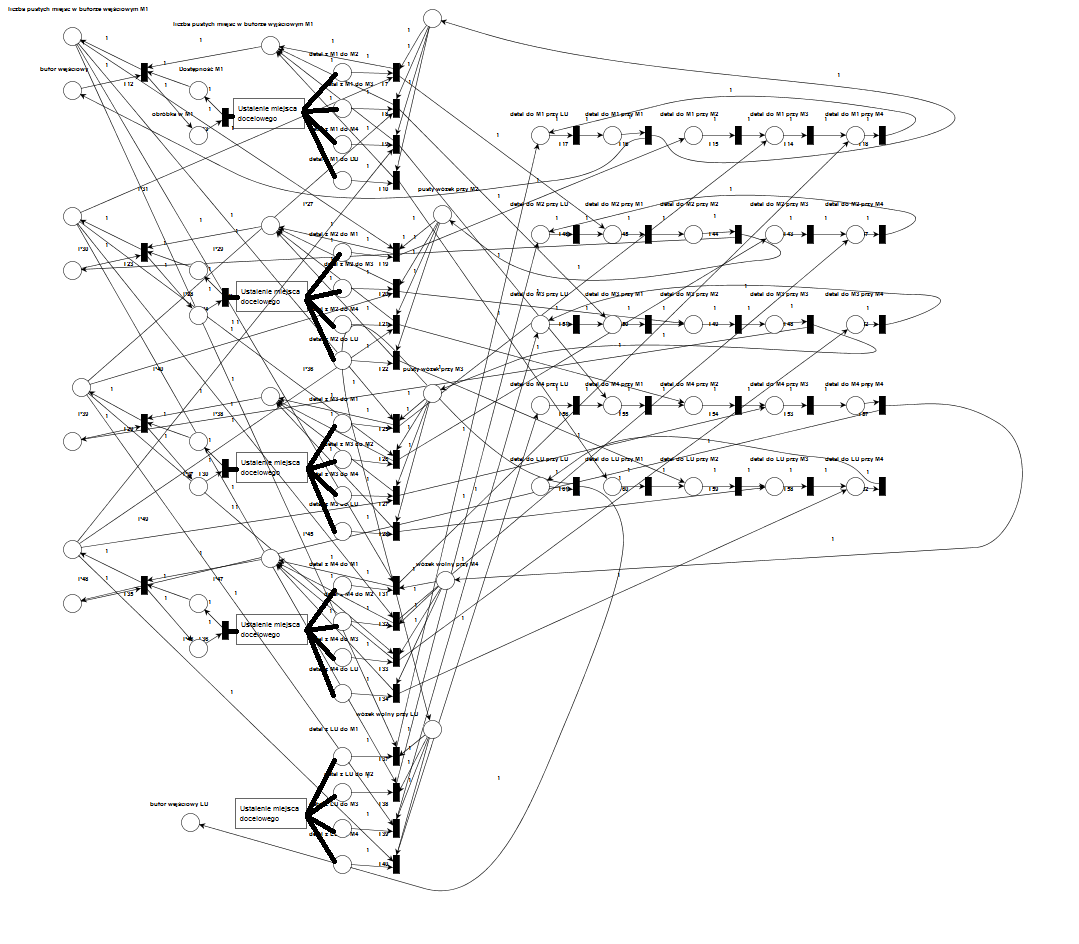
\includegraphics[width=1\textwidth]{./obrazki/Petri.png}
    \caption{Sieć Petriego}
    \label{fig:petri}
  \end{center}
 \end{figure}
Wykorzystaliśmy standardowe oznaczenia miejsc i tranzycji w sieciach Petriego. Wyróżniliśmy operacje maszynowe oraz realizowane przez wózki AGV, które są obserwowalne przez sterownik główny, po zakończeniu danego zadania maszyna/wózek informuje o tym kontroler główny, który może zlecić nowe zadanie dla maszyny/wózka (zdarzenie kontrolowalne).

\section{Plan pracy i rozkład w czasie}
\label{sec:org}

Na rysunku~\ref{fig:gantt} znajdują się wyselekcjonowane zadania oraz czas ich trwania jak również zaznaczone zostały kamienie milowe. 
 \begin{figure}[H]
  \begin{center}
    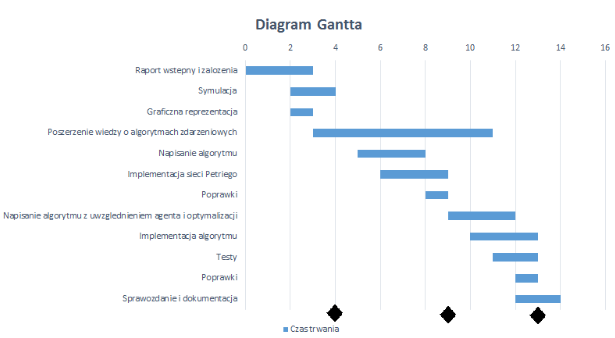
\includegraphics[width=1\textwidth]{./obrazki/gantt.png}
    \caption{Diagram Gantta}
    \label{fig:gantt}
  \end{center}
 \end{figure}

\section{Zarządzanie projektem}

Spotkania zespołu odbywać się będą w terminie zajęć oraz po wcześniejszym umówieniu się członków zespołu przy użyciu \textit{Skype’a} oraz grupy na portalu społecznościowym \textit{Facebook}. Oficjalnym liderem grupy jest Hanna Sienkiewicz. Jest to osoba, która jest odpowiedzialna za rozliczanie z zadań członków grupy przed upływem wyznaczonych terminów. Podział zadań w grupie następuje zgodnie z umiejętnościami i oczekiwaniami poszczególnych członków grupy. Nie przewidujemy problemów z tym związanych, członkowie grupy czują się zobligowani do pomocy przy większych i trudniejszych zadaniach. 

\section{Zespół}

W skład zespołu projektowego wchodzą
\begin{itemize}
\item Hanna Sienkiewicz, lider grupy, dane kontaktowe: 184184@student.pwr.edu.pl,
\item Marcin Ciopcia,
\item Daniel Gut,
\item Piotr Semberecki,
\item Mateusz Stachowski.
\end{itemize}

\section{Struktura systemu}

W systemie zdarzeniowym można wyróżnić
\begin{itemize}
\item sterownik główny,
\item sterowniki maszyn,
\item sieć Petrie'go,
\item symulator zdarzeń.
\end{itemize}

Symulator ma za zadanie zasymulować uruchomienie zadania na maszynie, ładowanie z bufora do maszyny oraz ładowania z maszyny na wózek.

Pierwszy model sterownika działa na zasadzie wykonywania zadań jako pierwszych, których suma czasów wykonywania poszczególnych etapów jest najmniejsza. Posiada on wiedzę o zadaniach, jakie mogą być wykonane w danym kroku czasowym oraz o maszynach, na których będą wykonywane poszczególne etapy zadania jaki o czasach wykonania poszczególnych etapów zadania.


Sieć (P/T Sieć) formalnie można zapisać za pomocą piątki $N\ =\ (P,\ T,\ F,\ W,\ M_0)$, gdzie:
\begin{itemize}
\item $P$ jest skończonym zbiorem miejsc,
\item $T$ jest skończonym zbiorem przejść (tranzycji),
\item $P \cap T =\ \{\o \}$ - zbiory miejsc i przejść są rozłączne,
\item $F \subseteq (P\times T)\cup (T\times P)$ jest relacją przepływu,
\item $W:F\to (\mathcal{N}-\{0\})$ jest funkcją wagi łuków,
\item $M_0:P  \to \mathcal{N}$ jest markowaniem początkowym.
\end{itemize}
\section{Sekwencyjny system alokacji zasobów}

RAS definiuje się jako piątkę $\Phi \ =\ (\mathcal{R},\ C,\ \mathcal{P},\ \mathcal{D},\ \mathcal{T})$, gdzie:
\begin{itemize}
\item $\mathcal{R}$ jest zbiorem typów zasobów,
\item $C$ jest funkcją pojemności zasobów,
\item $\mathcal{P}$ - jest zbiorem typów procesów,
\item $F \subseteq (P\times T)\cup (T\times P)$ jest relacją przepływu,
\item $W:F\to (\mathcal{N}-\{0\})$ jest funkcją wagi łuków.
\item $\mathcal{R}=\{M_i,\ B_{wy_i},\ B_{we_i},\ L/U,\ AGV_j,\ W_j\}$, $i=1,\dots 4,\ j=1,\dots, 4$, gdzie $M$ - zasób maszynowy, $B$ - zasób buforowy, $L/U$ - zasób stacji, $AGV$ - zasób wózków, $W$ - zasób wolnego miejsca między maszynami.
\item $C(M_i)=1,\ C(B_{we_i})=x,\ C(B_{wy_i})=y,\ C(AGV_i)=z,\ C(L/U)=\infty,\ C(W_j)=w;\ x,\ y,\ z,\ w$ - parametry,
\item $\mathcal{P}=\{\Pi_i\}$, $i=1,\dots, 6$, (6 procesów to 6 typów produktów),
\item $\Pi_j=\big<\mathcal{S}_j,\mathcal{G}_j\big>$,
\item $\mathcal{S}_j=\{Om_{j1},\dots ,Om_{jn(j)}, Ow_{j1},\dots ,Ow_{jm(j)} \}$ zbiór operacji procesu $\Pi_j$, $Om$ - operacje maszynowe, $Ow$ - operacje transportowe,
\item $\mathcal{G}_j=\{O, t\}$ jest strukturą danych wyznaczającą logikę wykonywania operacji procesu $\Pi_j$; $O$ to zbiór operacji, $t$ czas operacji $O$
\item $\mathcal{D}:$  jest funkcją wymagań zasobowych operacji, operacje transportu wymagają dostępności wózków oraz wolnej ścieżki między danymi maszynami, operację maszynowe wymagają miejsca w buforze wejściowym oraz wyjściowym jaki i dostępności maszyny; np. $D_{11}=\{B_we1,\ M_1,\ B_wy1\}$ - wymagania zasobowe operacji maszynowej $Om_{11}$.


\end{itemize}
SU-RAS, w którym funkcja wymagań zasobowych jest określona przez D. Każda operacja $O$ wymaga jednej jednostki jednego typu zasobu.

Jeżeli detal musi zostać przewieziony z bufora wyjściowego maszyny X na bufor wejściowy maszyny Y to żąda on wolnego miejsca na trasie miedzy tymi maszynami i jednocześnie wózka, który go przewiezie, to oznacza, że jeżeli wózek i wolne miejsce na trasie to zasoby to operacja transportu wymaga dwóch jednostek zasobów różnych typów (każda operacja wymaga jednej jednostki jednego typu zasobu).

\section{Unikanie blokad}
Bufory muszą mieć pojemność większą nić 1.


\section{Stan sieci}
Stan sieci to macierz rozmiaru $11$x$ 5$. Stan początkowy wygląda następująco
\begin{equation}
\left[\begin{array}{ccccc}
0 & 0 & 0 & 0&0\\
0 &0 &0 &0&0\\
0 &0 &0 &0&0\\
0 &0 &0 &0&0\\
0 &0 &0 &0&0\\
0 &0 &0 &0 &1\\
0 &0 &0 &0&0\\
b_{we}&b_{we}&b_{we}&b_{we} & \infty\\
b_{wy}&b_{wy}&b_{wy}&b_{wy} & \infty\\
1&1&1&1 &1\\
0 &0 &0 &0 &0
\end{array}\right],
\end{equation}
gdzie $b_{we}$, $b_{wy}$ to odpowiednio rozmiar bufora wejściowego i wyjściowego, a
\begin{itemize}
\item 1 wiersz sieci to transport do maszyny 1
\item 2 wiersz sieci to transport do maszyny 2
\item 3 wiersz sieci to transport do maszyny 3
\item 4 wiersz sieci to transport do maszyny 4
\item 5 wiersz sieci to transport do LU
\item 6 wiersz sieci to oznaczenie miejsca z pustym wókiem (domyslnie jeden pusty wozek przy LU)
\item 7 wiersz sieci to ilość detali w buforach wejściowych (domyślnie zero dla każdej maszyny)
\item 8 wiersz sieci to liczby pustych miejsc w buforach wejściowych dla każdej z maszyn
\item 9 wiersz sieci to liczby pustych miejsc w buforach wyjściowych dla każdej z maszyn
\item 10 wiersz sieci to dostępność maszyn (domyślnie wszystkie maszyny sa dostępne)
\item 11 wiersz sieci to obróbka na maszynie
\end{itemize}
Transport do maszyny nr 4 z maszyny nr 3 to S[4][3]=1. Po wykonaniu tego transportu mamy S[4][3]=0 oraz S[4][4]=1. Gdy następuje transport z maszyny nr 4 na maszynę nr 4 to mamy S[4][4]=0, S[7][4] = 1 (detal w buforze wejściowym maszyny nr 4) oraz S[6][4] = 1 (pusty wózek przy maszynie nr 4)
\section{Funkcje}
\label{funkcje}
Istnieją 4 typy zadań
\begin{itemize}

\item Typ 3 - Załaduj wózek,
Zgłaszamy, że detal nie jest już w gnieździe maszyny, maszyna ta staje się dostępna. Sprawdzamy czy mamy pusty wózek przy maszynie i czy jest miejsce w buforze wejściowym maszyny docelowej. Jeśli tak to rezerwujemy wózek. Zmniejszamy liczbę dostępnych miejsc w buforze wejściowym maszyny docelowej o 1. Zwiększamy miejsce w buforze wejściowym dla maszyny, która opuszcza detal. W wierszu o nr maszyny docelowej, zaznaczamy transport do niej począwszy od maszyny aktualnej. W takim stanie możliwy jest transport.
\begin{equation}
S_1=\left[\begin{array}{ccccc}
0 & 0 & 0 & 0&0\\
0 & 0 & 0 & 0 & 0\\
0 & 0 & 0 & 0& 0\\
0 & 0 & 0 & 0& 0\\
0 & 0 & 0 & 0& 0\\
1 & 0 & 0 & 0 & 0\\
0 & 0 & 0 & 0& 0\\
b_{we}& b_{we}& b_{we}& b_{we} & \infty\\
b_{wy}& b_{wy}& b_{wy}& b_{wy} & \infty\\
0& 1& 1& 1 & 1\\
1 & 0 & 0 & 0 & 0
\end{array}\right],
\end{equation}
$S_1[6][1]=1$ jest pusty wózek przy maszynie nr 1. $S_1[10][1]=0$ maszyna nie jest dostępna. $S_1[11][1]=0$ obróbka detalu trwa. $S_1[8][3]=1$ jest miejsce w buforze wejściowym maszyny docelowej transportu (w tym przykładnie maszyna nr 3). $S_1[8][3]>0$ bufor wejściowy maszyny docelowej nie jest pełny. Po zgłoszeniu zadania "Załaduj wózek" mamy
\begin{equation}
S_2=\left[\begin{array}{ccccc}
0 & 0 & 0 & 0&0\\
0 & 0 & 0 & 0 & 0\\
1 & 0 & 0 & 0& 0\\
0 & 0 & 0 & 0& 0\\
0 & 0 & 0 & 0& 0\\
0 & 0 & 0 & 0 & 0\\
0 & 0 & 0 & 0& 0\\
b_{we}& b_{we}& b_{we}-1& b_{we} & \infty\\
b_{wy}+1& b_{wy}& b_{wy}& b_{wy} & \infty\\
1& 1& 1& 1 & 1\\
0 & 0 & 0 & 0 & 0
\end{array}\right],
\end{equation}
$S_2[6][1]=0$ rezerwujemy wózek. $S_2[10][1]=1$ maszyna jest znów dostępna. $S_2[11][1]=0$ obróbka zakończona. $S_2[3][1]=1$ zaznaczamy transport z maszyny nr 1 na maszynę docelową (nr 3). $S_2[8][3]=b_{we}-1$ zmniejszamy liczbę dostępnych miejsc w buforze wejściowym maszyny docelowej. $S_2[9][1]=b_{wy}+1$ zwiększamy liczbę dostępnych miejsc w buforze wyjściowym maszyny nr 1. Możliwe jest zadanie transportu.

\item Typ 2 - Wykonaj transport(etap, nr maszyny docelowej),
\begin{equation}
S_3=\left[\begin{array}{ccccc}
0 & 0 & 0 & 0&0\\
0 & 0 & 0 & 0 & 0\\
0 & 1 & 0 & 0& 0\\
0 & 0 & 0 & 0& 0\\
0 & 0 & 0 & 0& 0\\
0 & 0 & 0 & 0 & 0\\
0 & 0 & 0 & 0& 0\\
b_{we}& b_{we}& b_{we}& b_{we} & \infty\\
b_{wy}& b_{wy}& b_{wy}& b_{wy} & \infty\\
1& 1& 1& 1 & 1\\
0 & 0 & 0 & 0 & 0
\end{array}\right],
\end{equation}
$S_3[3][1]=0$, $S_3[3][2]=1$ został wykonany transport z maszyny nr 1 na maszynę nr 2, dalej wykonujemy transport z maszyny nr 2 na maszynę nr 3.
\begin{equation}
S_4=\left[\begin{array}{ccccc}
0 & 0 & 0 & 0&0\\
0 & 0 & 0 & 0 & 0\\
0 & 0 & 1 & 0& 0\\
0 & 0 & 0 & 0& 0\\
0 & 0 & 0 & 0& 0\\
0 & 0 & 0 & 0 & 0\\
0 & 0 & 0 & 0& 0\\
b_{we}& b_{we}& b_{we}& b_{we} & \infty\\
b_{wy}& b_{wy}& b_{wy}& b_{wy} & \infty\\
1& 1& 1& 1 & 1\\
0 & 0 & 0 & 0 & 0
\end{array}\right],
\end{equation}
$S_4[3][2]=0$, $S_4[3][3]=1$ został wykonany transport z maszyny nr 2 na maszynę nr 3, dalej wykonujemy transport z "maszyny nr 3 na maszynę nr 3".
\begin{equation}
S_5=\left[\begin{array}{ccccc}
0 & 0 & 0 & 0&0\\
0 & 0 & 0 & 0 & 0\\
0 & 0 & 0 & 0& 0\\
0 & 0 & 0 & 0& 0\\
0 & 0 & 0 & 0& 0\\
0 & 0 & 1 & 0 & 0\\
0 & 0 & 1 & 0& 0\\
b_{we}& b_{we}& b_{we}& b_{we} & \infty\\
b_{wy}& b_{wy}& b_{wy}& b_{wy} & \infty\\
1& 1& 1& 1 & 1\\
0 & 0 & 0 & 0 & 0
\end{array}\right],
\end{equation}
$S_5[3][3]=0$, $S_5[6][3]=1$ mamy pusty wózek przy maszynie nr 3, $S_5[7][3]=1$ mamy detal w buforze wejściowym maszyny nr 3.
\item Typ 1 - Załaduj detal na maszynę,
Jeśli jest to ostatni etap zadania i maszyna docelowa to LU, to zadanie zostaje zakończone. Zgłaszamy pusty wózek. Zwiększamy liczbę miejsc w buforze wejściowym maszyny o 1. Zgłaszamy możliwość obróbki.
\begin{equation}
S_6=\left[\begin{array}{ccccc}
0 & 0 & 0 & 0&0\\
0 & 0 & 0 & 0 & 0\\
0 & 0 & 0 & 0& 0\\
0 & 0 & 0 & 0& 0\\
0 & 0 & 0 & 0& 0\\
0 & 0 & 1 & 0 & 0\\
0 & 0 & 0 & 0& 0\\
b_{we}& b_{we}& b_{we}+1& b_{we} & \infty\\
b_{wy}& b_{wy}& b_{wy}& b_{wy} & \infty\\
1& 1& 1& 1 & 1\\
0 & 0 & 0 & 0 & 0
\end{array}\right],
\end{equation}
$S_6[8][3]=b_{we}+1$ zwiększamy liczbę miejsc w buforze wejściowym maszyny o 1.


\item Typ 4 - Wykonaj obróbkę.
Do odpowiedniej kolumny wiersza 11 jest wpisywana jedynka. Zostaje zwolniony wózek. 
\begin{equation}
S_7=\left[\begin{array}{ccccc}
0 & 0 & 0 & 0&0\\
0 & 0 & 0 & 0 & 0\\
0 & 0 & 0 & 0& 0\\
0 & 0 & 0 & 0& 0\\
0 & 0 & 0 & 0& 0\\
0 & 0 & 1 & 0 & 0\\
0 & 0 & 0 & 0& 0\\
b_{we}& b_{we}& b_{we}& b_{we} & \infty\\
b_{wy}& b_{wy}& b_{wy}& b_{wy} & \infty\\
0 & 1& 1& 1 & 1\\
1 & 0 & 0 & 0 & 0
\end{array}\right],
\end{equation}
$S_7[11][3]=1$ obróbka na maszynie nr 3. $S_7[10][3]=0$ maszyna nr 3 nie jest wolna. Zgłaszamy możliwość załadunku wózka, po wykonanej obróbce.
\end{itemize}
\section{Opis sterowania}
Rysunek nr~\ref{fig:alg} przedstawia działanie modelu zdarzeniowego.
 \begin{figure}[H]
  \begin{center}
    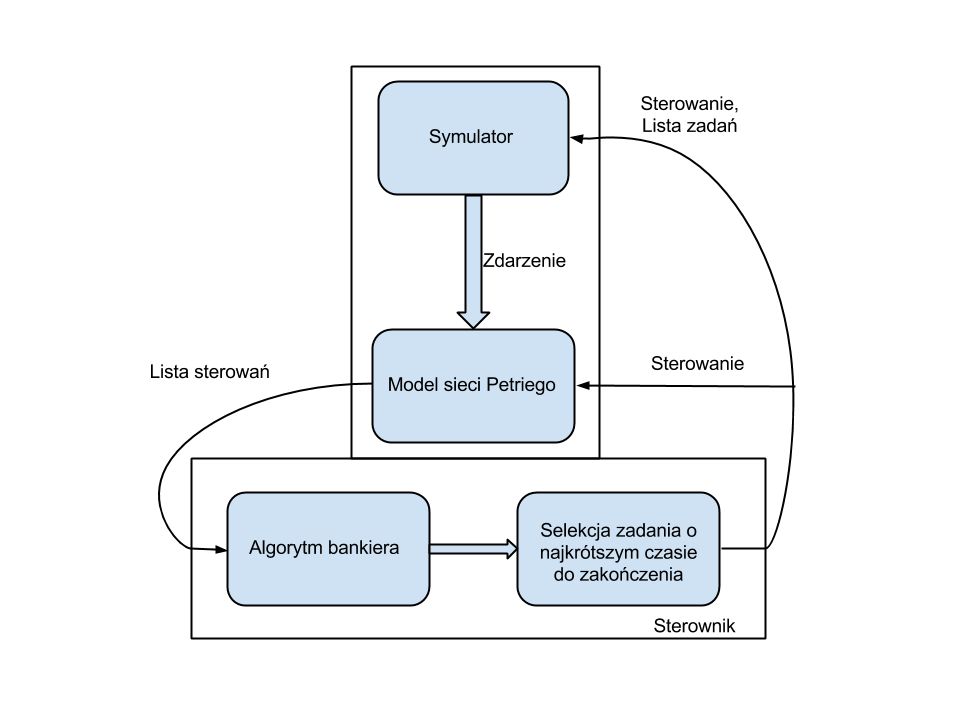
\includegraphics[width=1\textwidth]{./obrazki/alg.png}
    \caption{Architektura sterownika}
    \label{fig:alg}
  \end{center}
 \end{figure}
\subsection{Inicjalizacja zadań}
Zadanie to struktura wchodząca w skład listy zadań składająca się z
\begin{itemize}
\item  numerów maszyn, na których są wykonywane poszczególne etapy zadań\\
\textit{Lista\_zadan(i).maszyny = [$M_j$, $\dots$,  $M_n$]},
\item czasów obróbki jednego detalu na maszynie\\
\textit{Lista\_zadan(i).czasy = [$t_j$, $\dots$,  $t_n$]},
\item liczby detali oczekujących na obróbkę na maszynie\\
\textit{Lista\_zadan(i).ilosc   = [k, $\dots$, 0]}.
\label{lista_zad}
\end{itemize}
\subsection{Sterownik}
Sterownik na podstawie listy dostępnych sterowań wygenerowanych przez model sieci Petriego, listy zadań oraz wielkości buforów wyjściowych i wejściowych maszyn generuje \textbf{Sterowanie}. \textbf{Sterowanie} to struktura zawierająca w sobie
\begin{itemize}
\item typ zadania (typy zadań zostały opisane w sekcji~\ref{funkcje}),
\item numer maszyny - określa nr maszyny, przy której zdarzenie wystąpiło,
\item numer - to numer zadania z listy zadań,
\item etap - to numer etapu zadania.
\end{itemize}
Sterowanie generowane jest poprzez algorytm bankiera, następnie z pośród możliwych zadań wybierane jest to, które ma najkrótszy czas do zakończenia. Algorytm bankiera jest zaimplementowany dla maszyn z zadania.  Agent przyjmuje jako parametry
\begin{itemize}
\item listę dostępnych sterowań wygenerowaną przez model sieci Petriego, zawierającą możliwe \textbf{Sterowania},
\item listę zadań.
\end{itemize}

\begin{thebibliography}{9}
\bibitem{scr}
  S. Samolej, B. Trybus,
  \emph{Zastosowanie kolorowanych sieci Petriego w projektowaniu systemów czasu rzeczywistego}.
  Pomiary, Automatyka, Kontrola,
  2005,
  tom R. 51, nr 1,
  11-13.
\bibitem{sl}  
  I. Grobelna, M. Grobelny,
  \emph{Projektowanie sterowników logicznych z wykorzystaniem łuków zezwalających i zakazujących sieci Petriego}.	
  Pomiary, Automatyka, Kontrola,
  2012,
  tom R. 58, nr 7,
  605-607.
  
 \bibitem{mucha} 
  G. Bocewicz, W. Muszyński, Z. Banaszak,
  \emph{Modele multimodalnych sieci i procesów transportowych}.
  Postępy robotyki pod redakcją K. Tchonia i C. Zielińskiego,
  Oficyna wydawnicza Politechniki Warszawskiej,
   Warszawa 2014,
   tom 2, s. 543-552.

\end{thebibliography}

\end{document}


 
